\section{Lookup Tables (Luts)}
An interesting approach to build a sort of network without backprop is described in \cite{chatterjee2018learning}. The input is a $d$-dimensional boolean vector and the output is either 0 or 1. The basic idea is to build a \enquote{lookup table} (lut) based on the training data. Many lookup tables (luts) are created and stacked, reminding us of a neural network. The paper shows that this architecture not only generalizes on yet unseen data, but also shares some properties of neural networks. Let us first start with the definition of a single lut and then work our way up to a netowrk of luts. We then discuss experimental results of \cite{chatterjee2018learning} which we also re-create on our own.

\subsection{Single Lookup Tables (Luts)}
Imagine the task is to classify a 2-bit input $\bm{x}$ into either 0 or 1. Since $\bm{x}$ has 2 bits, $\bm{x} \in \{00, 01, 10, 11 \}$. Given training data $(\bm{X}, \bm{y})$, where $\bm{X}$ has $N$ rows and 2 columns and $\bm{y}$ has $N$ rows and 1 column, we are tasked with creating a lut $f$:

\begin{align}
    f(\bm{x}) = \begin{cases}
        ? \quad \text{if} \quad \bm{x} = 00, \\
        ? \quad \text{if} \quad \bm{x} = 01, \\
        ? \quad \text{if} \quad \bm{x} = 10, \\
        ? \quad \text{if} \quad \bm{x} = 11. \\
    \end{cases}
\end{align} If the training data has 90 examples of $01$ with the label 1, and 10 examples of $01$ with the label 0, it makes sense for any new unseen $\bm{x}$ to be classified with label 1. Our lut $f$ now looks like this:

\begin{align}
    f(\bm{x}) = \begin{cases}
        ? \quad \text{if} \quad \bm{x} = 00, \\
        1 \quad \text{if} \quad \bm{x} = 01, \\
        ? \quad \text{if} \quad \bm{x} = 10, \\
        ? \quad \text{if} \quad \bm{x} = 11. \\
    \end{cases}
\end{align} As we have seen, the basic idea is to count occurrences: for any bit pattern we count how many times it has the label 0 and how many times it has the label 1 and plug into the lut the value which occurrs most often. But what if a bit pattern has an equal number of examples for $y=0$ and $y=1$? That also includes the bit pattern not occurring in the training set at all. We call such circumstances \enquote{ties} and in order to break them, we assign in the lut a random entry for that bit pattern. Going back to our example, suppose for the pattern $(11)$ there are 50 training exapmles with label 1 and 50 training examples with label 0. We randomly sample a value from $\{0, 1\}$, obtaining 0. The lut now looks like this:

\begin{empheq}[left={f(\bm{x})=\empheqlbrace}]{equation}\begin{alignedat}{2}
    & 0^* \quad & \text{if} & \quad \bm{x} = 00, \\
    & 1 \quad & \text{if} & \quad \bm{x} = 01, \\
    & ? \quad & \text{if} & \quad \bm{x} = 10, \\
    & ? \quad & \text{if} & \quad \bm{x} = 11, \\
\end{alignedat}
\end{empheq} where we have denoted the random lut entry with a $*$. The following example demonstrates constructing a 3-bit lut.

\begin{example}\label{ex:1}
    Given 3-bit dataset $\bm{X}$ with labels $y$, we are tasked with creating a lut which assigns either 0 or 1 to a bit pattern. For each bit pattern, we count how many times $y=0$ and $y=1$ and choose the value which occurrs more often as final classification. In the case of ties, we assign a random value, denoted by a $*$.

\small
\begin{minipage}{.95\linewidth}\centering
  \begin{minipage}[b]{.2\linewidth}\centering
    Training set
    \begin{align*}
      \begin{array}{cc}
        \bm{X}                         & y                      \\ \hline
        \multicolumn{1}{|c|}{000} & \multicolumn{1}{c|}{0} \\ \hline
        \multicolumn{1}{|c|}{000} & \multicolumn{1}{c|}{1} \\ \hline
        \multicolumn{1}{|c|}{000} & \multicolumn{1}{c|}{1} \\ \hline
        \multicolumn{1}{|c|}{001} & \multicolumn{1}{c|}{1} \\ \hline
        \multicolumn{1}{|c|}{100} & \multicolumn{1}{c|}{0} \\ \hline
        \multicolumn{1}{|c|}{110} & \multicolumn{1}{c|}{0} \\ \hline
        \multicolumn{1}{|c|}{110} & \multicolumn{1}{c|}{1} \\ \hline
      \end{array}
    \end{align*}
  \end{minipage}
  \begin{minipage}[b]{.4\linewidth}\centering
    \begin{align*}
      \begin{array}{ccc}
        \text{bit pattern}        & \sum\limits_{y=0}      & \multicolumn{1}{l}{\sum\limits_{y=1}} \\ \hline
        \multicolumn{1}{|c|}{000} & \multicolumn{1}{c|}{1} & \multicolumn{1}{c|}{2}                \\ \hline
        \multicolumn{1}{|c|}{001} & \multicolumn{1}{c|}{0} & \multicolumn{1}{c|}{1}                \\ \hline
        \multicolumn{1}{|c|}{010} & \multicolumn{1}{c|}{0} & \multicolumn{1}{c|}{0}                \\ \hline
        \multicolumn{1}{|c|}{011} & \multicolumn{1}{c|}{0} & \multicolumn{1}{c|}{0}                \\ \hline
        \multicolumn{1}{|c|}{100} & \multicolumn{1}{c|}{1} & \multicolumn{1}{c|}{0}                \\ \hline
        \multicolumn{1}{|c|}{101} & \multicolumn{1}{c|}{0} & \multicolumn{1}{c|}{0}                \\ \hline
        \multicolumn{1}{|c|}{110} & \multicolumn{1}{c|}{1} & \multicolumn{1}{c|}{1}                \\ \hline
        \multicolumn{1}{|c|}{111} & \multicolumn{1}{c|}{0} & \multicolumn{1}{c|}{0}                \\ \hline
      \end{array}
    \end{align*}
  \end{minipage}
  \begin{minipage}[b]{.3\linewidth}\centering
    \begin{align*}
      \begin{array}{cc}
        \text{bit pattern}        & f                  \\ \hline
        \multicolumn{1}{|c|}{000} & \multicolumn{1}{l|}{1}   \\ \hline
        \multicolumn{1}{|c|}{001} & \multicolumn{1}{l|}{1}   \\ \hline
        \multicolumn{1}{|c|}{010} & \multicolumn{1}{l|}{0^*} \\ \hline
        \multicolumn{1}{|c|}{011} & \multicolumn{1}{l|}{1^*} \\ \hline
        \multicolumn{1}{|c|}{100} & \multicolumn{1}{l|}{0}   \\ \hline
        \multicolumn{1}{|c|}{101} & \multicolumn{1}{l|}{1^*}  \\ \hline
        \multicolumn{1}{|c|}{110} & \multicolumn{1}{l|}{1^*}  \\ \hline
        \multicolumn{1}{|c|}{111} & \multicolumn{1}{l|}{0^*} \\ \hline
      \end{array}
    \end{align*}
  \end{minipage}
\end{minipage}
  \normalfont
\end{example}
\qed

\noindent In \cite{chatterjee2018learning}, it is shown that a learned lut is the best we can do given the training set, meaning no other learning scheme will yield a classifier with higher accuracy. However, a single lut cannot do much. It makes sense intuitively that a single lookup table cannot capture complex relationships. Moreover, single luts become impractical with increasing bit size. For example, a very small image of size $28 \times 28$ has $28 \cdot 28 = 784$ entries. A 784-lut would need to have $2^{784} \propto 10^{236}$ entries which is computationally infeasible. Any two images, even with very similar content, will most likely never be the same to the pixel, rendering the lut learning algorithm useless. In the following section we will look at how to construct a network of multiple luts which will be able to handle more bits and learn complex relationships.

\subsection{Network of Lookup Tables (Luts)}
We will now demonstrate the scheme to construct a lut network according to \cite{chatterjee2018learning}. Consider the dataset from Example~\ref{ex:1}. Instead of constructing a lut that utilizes all bits, we now take \textbf{random} subsets of the columns. If $\bm{X} = \{x_0,x_1,x_2\}$, where $x_j$ are the individual conlumns of $\bm{X}$, then we consider $\{x_0,x_1\}$ and $\{x_0,x_2\}$. We obtain two matrices with 7 rows (same as before), but only 2 columns instead of 3. With these 2 matrices we can construct two luts, using the \textbf{same} label vector $y$. The matrices and new luts can be seen in Figure~\ref{fig:ex1}.

\begin{figure}[!htb]
\small
\begin{minipage}{.95\linewidth}\centering
  \begin{minipage}[b]{.19\linewidth}\centering
    Training set
    \vspace{-0.5em}
    \begin{align*}
      \begin{array}{cc}
        \{x_0,x_1\}                    & y                      \\ \hline
        \multicolumn{1}{|c|}{00} & \multicolumn{1}{c|}{0} \\ \hline
        \multicolumn{1}{|c|}{00} & \multicolumn{1}{c|}{1} \\ \hline
        \multicolumn{1}{|c|}{00} & \multicolumn{1}{c|}{1} \\ \hline
        \multicolumn{1}{|c|}{00} & \multicolumn{1}{c|}{1} \\ \hline
        \multicolumn{1}{|c|}{10} & \multicolumn{1}{c|}{0} \\ \hline
        \multicolumn{1}{|c|}{11} & \multicolumn{1}{c|}{0} \\ \hline
        \multicolumn{1}{|c|}{11} & \multicolumn{1}{c|}{1} \\ \hline
      \end{array}
    \end{align*}
  \end{minipage}
  \begin{minipage}[b]{.4\linewidth}\centering
    \begin{align*}
      \begin{array}{cccc}
          \text{bit pattern}        & \sum\limits_{y=0}      & \multicolumn{1}{l}{\sum\limits_{y=1}} & f_0  \\ \hline
        \multicolumn{1}{|c|}{00} & \multicolumn{1}{c|}{1} & \multicolumn{1}{c|}{3} & \multicolumn{1}{l|}{1} \\ \hline
        \multicolumn{1}{|c|}{01} & \multicolumn{1}{c|}{0} & \multicolumn{1}{c|}{0} & \multicolumn{1}{l|}{1^*} \\ \hline
        \multicolumn{1}{|c|}{10} & \multicolumn{1}{c|}{1} & \multicolumn{1}{c|}{0} & \multicolumn{1}{l|}{0} \\ \hline
        \multicolumn{1}{|c|}{11} & \multicolumn{1}{c|}{1} & \multicolumn{1}{c|}{1} & \multicolumn{1}{l|}{1^*} \\ \hline
      \end{array}
    \end{align*}
  \end{minipage}
  \begin{minipage}[b]{.21\linewidth}\centering
    Prediction on training set
    \vspace{-0.5em}
    \begin{align*}
      \begin{array}{cc}
        \{x_0,x_1\}                    & f_0(\bm{x})              \\ \hline
        \multicolumn{1}{|c|}{00} & \multicolumn{1}{c|}{1} \\ \hline
        \multicolumn{1}{|c|}{00} & \multicolumn{1}{c|}{1} \\ \hline
        \multicolumn{1}{|c|}{00} & \multicolumn{1}{c|}{1} \\ \hline
        \multicolumn{1}{|c|}{00} & \multicolumn{1}{c|}{1} \\ \hline
        \multicolumn{1}{|c|}{10} & \multicolumn{1}{c|}{0} \\ \hline
        \multicolumn{1}{|c|}{11} & \multicolumn{1}{c|}{1} \\ \hline
        \multicolumn{1}{|c|}{11} & \multicolumn{1}{c|}{1} \\ \hline
      \end{array}
    \end{align*}
  \end{minipage}
\end{minipage}

\begin{minipage}{.95\linewidth}\centering
  \begin{minipage}[b]{.19\linewidth}\centering
    Training set
    \vspace{-0.5em}
    \begin{align*}
      \begin{array}{cc}
        \{x_0,x_2\}                    & y                      \\ \hline
        \multicolumn{1}{|c|}{00} & \multicolumn{1}{c|}{0} \\ \hline
        \multicolumn{1}{|c|}{00} & \multicolumn{1}{c|}{1} \\ \hline
        \multicolumn{1}{|c|}{00} & \multicolumn{1}{c|}{1} \\ \hline
        \multicolumn{1}{|c|}{01} & \multicolumn{1}{c|}{1} \\ \hline
        \multicolumn{1}{|c|}{10} & \multicolumn{1}{c|}{0} \\ \hline
        \multicolumn{1}{|c|}{10} & \multicolumn{1}{c|}{0} \\ \hline
        \multicolumn{1}{|c|}{10} & \multicolumn{1}{c|}{1} \\ \hline
      \end{array}
    \end{align*}
  \end{minipage}
  \begin{minipage}[b]{.4\linewidth}\centering
    \begin{align*}
      \begin{array}{cccc}
          \text{bit pattern}        & \sum\limits_{y=0}      & \multicolumn{1}{l}{\sum\limits_{y=1}} & f_1  \\ \hline
        \multicolumn{1}{|c|}{00} & \multicolumn{1}{c|}{1} & \multicolumn{1}{c|}{2} & \multicolumn{1}{l|}{1} \\ \hline
        \multicolumn{1}{|c|}{01} & \multicolumn{1}{c|}{0} & \multicolumn{1}{c|}{1} & \multicolumn{1}{l|}{1} \\ \hline
        \multicolumn{1}{|c|}{10} & \multicolumn{1}{c|}{2} & \multicolumn{1}{c|}{0} & \multicolumn{1}{l|}{0} \\ \hline
        \multicolumn{1}{|c|}{11} & \multicolumn{1}{c|}{0} & \multicolumn{1}{c|}{0} & \multicolumn{1}{l|}{1^*} \\ \hline
      \end{array}
    \end{align*}
  \end{minipage}
  \begin{minipage}[b]{.21\linewidth}\centering
      \vspace{1em}
    Prediction on training set
    \vspace{-0.5em}
    \begin{align*}
      \begin{array}{cc}
        \{x_0,x_2\}                    & f_1(\bm{x})              \\ \hline
        \multicolumn{1}{|c|}{00} & \multicolumn{1}{c|}{1} \\ \hline
        \multicolumn{1}{|c|}{00} & \multicolumn{1}{c|}{1} \\ \hline
        \multicolumn{1}{|c|}{00} & \multicolumn{1}{c|}{1} \\ \hline
        \multicolumn{1}{|c|}{01} & \multicolumn{1}{c|}{1} \\ \hline
        \multicolumn{1}{|c|}{10} & \multicolumn{1}{c|}{0} \\ \hline
        \multicolumn{1}{|c|}{10} & \multicolumn{1}{c|}{0} \\ \hline
        \multicolumn{1}{|c|}{10} & \multicolumn{1}{c|}{0} \\ \hline
      \end{array}
    \end{align*}
  \end{minipage}
\end{minipage}
  \normalfont
  \caption{Two subsets of columns of the original dataset from Example~\ref{ex:1} that are the basis for 2 new luts. Note that the label vector $y$ is the \textbf{same} for both luts.}
    \label{fig:ex1}
\end{figure}
\FloatBarrier

\noindent What we have now are two separate luts, but we would like to construct a network. In order to do that, we apply each lut on the dataset it was trained on and stack the predictions horizontally. The stacked predictions, along with the original label column $y$, form a new dataset on which we can train a third lut. This process is visible in Figure~\ref{fig:ex2}.

\begin{figure}[!htb]
\small
\begin{minipage}{.95\linewidth}\centering
  \begin{minipage}[b]{.21\linewidth}\centering
    \begin{align*}
      \begin{array}{cc}
        \{x_0,x_1\}                    & f_0(\bm{x})              \\ \hline
        \multicolumn{1}{|c|}{00} & \multicolumn{1}{c|}{1} \\ \hline
        \multicolumn{1}{|c|}{00} & \multicolumn{1}{c|}{1} \\ \hline
        \multicolumn{1}{|c|}{00} & \multicolumn{1}{c|}{1} \\ \hline
        \multicolumn{1}{|c|}{00} & \multicolumn{1}{c|}{1} \\ \hline
        \multicolumn{1}{|c|}{10} & \multicolumn{1}{c|}{0} \\ \hline
        \multicolumn{1}{|c|}{11} & \multicolumn{1}{c|}{1} \\ \hline
        \multicolumn{1}{|c|}{11} & \multicolumn{1}{c|}{1} \\ \hline
      \end{array}
    \end{align*}
  \end{minipage}
  \begin{minipage}[b]{.1\linewidth}\centering
      +
      \vspace{4em}
  \end{minipage}
  \begin{minipage}[b]{.21\linewidth}\centering
    \begin{align*}
      \begin{array}{cc}
        \{x_0,x_2\}                    & f_1(\bm{x})      \\ \hline
        \multicolumn{1}{|c|}{00} & \multicolumn{1}{c|}{1} \\ \hline
        \multicolumn{1}{|c|}{00} & \multicolumn{1}{c|}{1} \\ \hline
        \multicolumn{1}{|c|}{00} & \multicolumn{1}{c|}{1} \\ \hline
        \multicolumn{1}{|c|}{01} & \multicolumn{1}{c|}{1} \\ \hline
        \multicolumn{1}{|c|}{10} & \multicolumn{1}{c|}{0} \\ \hline
        \multicolumn{1}{|c|}{10} & \multicolumn{1}{c|}{0} \\ \hline
        \multicolumn{1}{|c|}{10} & \multicolumn{1}{c|}{0} \\ \hline
      \end{array}
    \end{align*}
  \end{minipage}
  \begin{minipage}[b]{.1\linewidth}\centering
      =
      \vspace{4em}
  \end{minipage}
  \begin{minipage}[b]{.21\linewidth}\centering
    \begin{align*}
      \begin{array}{cc}
        f_0(\bm{x})                    & f_1(\bm{x})      \\ \hline
        \multicolumn{1}{|c|}{1} & \multicolumn{1}{c|}{1} \\ \hline
        \multicolumn{1}{|c|}{1} & \multicolumn{1}{c|}{1} \\ \hline
        \multicolumn{1}{|c|}{1} & \multicolumn{1}{c|}{1} \\ \hline
        \multicolumn{1}{|c|}{1} & \multicolumn{1}{c|}{1} \\ \hline
        \multicolumn{1}{|c|}{0} & \multicolumn{1}{c|}{0} \\ \hline
        \multicolumn{1}{|c|}{1} & \multicolumn{1}{c|}{0} \\ \hline
        \multicolumn{1}{|c|}{1} & \multicolumn{1}{c|}{0} \\ \hline
      \end{array}
    \end{align*}
  \end{minipage}
\end{minipage}

\begin{minipage}{.95\linewidth}\centering
  \begin{minipage}[b]{.30\linewidth}\centering
    \begin{align*}
      \begin{array}{cc}
        \{f_0(\bm{x}),f_1(\bm{x})\}          & y          \\ \hline
        \multicolumn{1}{|c|}{11} & \multicolumn{1}{c|}{0} \\ \hline
        \multicolumn{1}{|c|}{11} & \multicolumn{1}{c|}{1} \\ \hline
        \multicolumn{1}{|c|}{11} & \multicolumn{1}{c|}{1} \\ \hline
        \multicolumn{1}{|c|}{11} & \multicolumn{1}{c|}{1} \\ \hline
        \multicolumn{1}{|c|}{00} & \multicolumn{1}{c|}{0} \\ \hline
        \multicolumn{1}{|c|}{10} & \multicolumn{1}{c|}{0} \\ \hline
        \multicolumn{1}{|c|}{10} & \multicolumn{1}{c|}{1} \\ \hline
      \end{array}
    \end{align*}
  \end{minipage}
  \begin{minipage}[b]{.4\linewidth}\centering
    \begin{align*}
      \begin{array}{cccc}
          \text{bit pattern}        & \sum\limits_{y=0}      & \multicolumn{1}{l}{\sum\limits_{y=1}} & f_2  \\ \hline
        \multicolumn{1}{|c|}{00} & \multicolumn{1}{c|}{1} & \multicolumn{1}{c|}{0} & \multicolumn{1}{l|}{0} \\ \hline
        \multicolumn{1}{|c|}{01} & \multicolumn{1}{c|}{0} & \multicolumn{1}{c|}{0} & \multicolumn{1}{l|}{1^*} \\ \hline
        \multicolumn{1}{|c|}{10} & \multicolumn{1}{c|}{1} & \multicolumn{1}{c|}{1} & \multicolumn{1}{l|}{0^*} \\ \hline
        \multicolumn{1}{|c|}{11} & \multicolumn{1}{c|}{1} & \multicolumn{1}{c|}{3} & \multicolumn{1}{l|}{1} \\ \hline
      \end{array}
    \end{align*}
  \end{minipage}
\end{minipage}
  \normalfont
  \caption{Training of $f_2$, the final lut. Predictions of $f_0$ and $f_1$ on the original dataset are stacked horizontally and form a new dataset, along with the original label vector $y$.}
    \label{fig:ex2}
\end{figure}
\FloatBarrier

\noindent With the final lut visible in Figure~\ref{fig:ex2} we have a \textit{network} which might not be evident looking at just tables. Figure~\ref{fig:first_lut_network} provides a visualization.

\begin{figure}[!htb]
    \centering
  \begin{minipage}[b]{.4\linewidth}
    \begin{tabular}{clll}
    bit pattern & $f_0$ & $f_1$ & $f_2$ \\ \hline
    00          & 1      & 1      & 0     \\
    01          & $1^*$  & 1      & $1^*$ \\
    10          & 0      & 0      & $0^*$ \\
    11          & $1^*$  & $1^*$ & 1    
    \end{tabular}
    \vspace{1.5em}
  \end{minipage}
    \includestandalone[]{standalone/first_lut_network}
\caption{A small 2-lut network. The inputs $x_j$ get fed into the first two luts and their predictions is the input to the last lut. Note that unlike in neural networks, the neurons are not fully connected, but connections are sparse.}
\label{fig:first_lut_network}
\end{figure}

\noindent The aforementioned example was very small. In practice, we will consider much higher dimensional datasets. There are several parameters which we have to choose when constructing a lut network, which are

\vspace{0.5em}
\setlist{nolistsep}
\begin{enumerate}
    \item the bit size of the individual luts,
    \item the number of hidden layers and
    \item the number of luts per hidden layer.
\end{enumerate}

\noindent One important thing to note is that the output layer is just one lut because in the end we want to obtain either 0 or 1. If, for example, each lut in the network has 8 bits and in the second to last layer there are 500 luts, then the outputs of 492 luts in the second to last layer will not be used for the final prediction. We could see this as wasting computation which is acknowledged in \cite{chatterjee2018learning}. In a later section, we will tackle the question whether an architecture where the outputs of all luts are used has any advantages.

What we described so far is the complete scheme to construct a lut network and we are ready for some experiments. Figure~\ref{fig:lut_algo} gives a an overview of the algorithm.

\begin{figure}[!htb]
\begin{tcolorbox}[colback=white]
    \textbf{Lut algorithm according to \cite{chatterjee2018learning}}
    \vspace{0.5em}

    \textit{Task:} Given binary dataset $\boldsymbol{X}$ (binary meaning entries are either 0 or 1) with $N$ rows and $d$ columns and binary label vector $y$ with $N$ entries, construct a lut network that takes a $d$-dimensional binary vector and classifies it with either 0 or 1
    \vspace{0.5em}

    \setlist{nolistsep}
    \begin{enumerate}
        \item Choose hyperparemters:
            \begin{itemize}
                \item Bit size (number of arguments) $\delta$ of individual luts, where $\delta \leq d$
                \item Number of hidden layers $L$
                \item Number of luts per hidden layer $l_1, l_2, \dots, l_L$
            \end{itemize}
        \item For $i=1, \dots, L$ do:
            \begin{itemize}
                \item For $j=1, \dots, l_i$ do:
                    \begin{itemize}
                        \item Randomly choose $\delta$ columns from the previous layer
                        \item For each of the $2^\delta$ bit patterns:
                            \begin{itemize}
                                \item Count how many times $y=0$
                                \item Count how many times $y=1$
                                \item Choose the label that occurs most often, random if they are the same
                            \end{itemize}
                    \end{itemize}
                \item Propagate, obtaining new dataset with same labels
            \end{itemize}
        \item Create lut in the last layer
    \end{enumerate}
\end{tcolorbox}
\caption{Lut algorithm according to \cite{chatterjee2018learning}.}
\label{fig:lut_algo}
\end{figure}

\subsection{Experiments with Lookup Tables (luts)}
In this section, we recreate several experiments from \cite{chatterjee2018learning} and compare our results to theirs. The MNIST dataset \cite{mnist} is used. It consists of 28x28 grayscale images of handwritten digits from 0-9 and has 60000 training examples and 10000 testing examples. Before we can use this dataset, we have to modify it. The labels range from 0-9, but a lut network is only able to output 0 or 1 as classification. Thus we define the task to distinguish between numbers 0-4 (label 0) and nubmers 5-9 (label 1). The inputs to a lut network also have be either 0 or 1, so we must binarize the dataset. We transform the data such that the minimum value becomes 0 and the maximum value becomes 1. Applying the operator $>1/2$, we obtain binary values. Figure~\ref{fig:mnist_dataset} shows several images of the original and binarized dataset.

\begin{figure}[!htb]
    \centering
  \begin{minipage}[b]{.4\linewidth}
      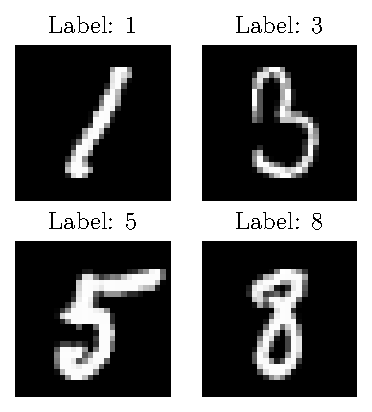
\includegraphics[width=.9\linewidth]{images/mnist_raw.pdf}
      \subcaption{Original.}
      \label{fig:mnist_dataset_original}
  \end{minipage}
  \begin{minipage}[b]{.4\linewidth}
      
\includegraphics[width=.9\linewidth]{images/mnist_binarized.pdf}
      \subcaption{Binarized.}
      \label{fig:mnist_dataset_binarized}
  \end{minipage}
  \caption{Samples from the original (\subref{fig:mnist_dataset_original}) and binarized (\subref{fig:mnist_dataset_binarized}) MNIST dataset. A lut network can only do binary classification, so we have to binarize the labels as well. Numbers from 0-4 get the label 0 and numbers from 5-9 get the label 1.}
\label{fig:mnist_dataset}
\end{figure}

\subsubsection{Lut Experiment 1}
We construct a lut network with 5 hidden layers of 1024 luts and 1 lut in the output layer. Every lut in the network takes 8 bits as input. Construction of the network is performed with the training set with 60000 samples and after training we validate on the test set with 10000 samples. We obtain a training accuracy of 0.89 and a test accuracy of 0.87 which are the exact results from \cite{chatterjee2018learning}. Note that the results are way above 0.5 meaning some learning had taken place. The way the lut network is defined, every does already a prediction on the example passed to the network. That means we can compute the training (or testing) accuracy for every lut in the network. Figure~\ref{fig:ex1_depth_performance} visualizes the training accuracy dependent on the layer. Each point represents the mean training accuracy over the respective layer and the total height of the error bars are two standard deviations. We can see that with increasing layer number, the accuracy goes up and the standard deviation goes down until it reaches 0 at layer number 6 because there is only 1 lut in the last layer. Increasing performance with increasing depth reminds us of neural networks where adding more layers is a heuristic to increase performance.

\begin{figure}[!htb]
    \centering
    \includestandalone[]{standalone/depth_performance}
    \caption{Training accuracy dependent on layer for an 8-lut network with 5 hidden layers (6 is the output layer with just one lut) and 1024 luts per layer, trained on the binary MNIST dataset. The points represent the mean over the respective layer with 2 standard deviations as total height of the error bars. Similar to neural networks, we can see that performance increases with increasing depth.}
\label{fig:ex1_depth_performance}
\end{figure}

The bit size of the luts (denoted by $\delta$ in Figure~\ref{fig:lut_algo}) is a crucial hyperparameter. In Figure~\ref{fig:ex1_k_acc} we vary the bit size from 2 to 16 with steps of 2 and observe the effect on training and test accuracy. The rest of the lut network is the same as before.

\begin{figure}[!htb]
    \centering
    \includestandalone[]{standalone/k_acc_real}
    \caption{k acc.}
\label{fig:ex1_k_acc}
\end{figure}
